\documentclass{beamer}

\mode<presentation>
{
  \usetheme{Marburg}
  \setbeamercovered{transparent}
  \usecolortheme{orchid}
}

\usepackage[english]{babel}
\usepackage[utf8]{inputenc}
\usepackage[T1]{fontenc} % Or whatever. Note that the encoding and the font should match. If T1
                         % does not look nice, try deleting the line with the fontenc.

\usepackage{amsmath}
\usepackage{mathtools}
\usepackage{lipsum}

\usepackage{tikz}
\usetikzlibrary{shapes,arrows}
\usepackage{pgfplots}
\usepackage{fancybox}

\title{Cryptocurrency Stabilization}
\subtitle{UCL Cryptocurrency Seminar}
\author{Robert Sams} 
\date{23 April 2015}
\subject{cryptocurrency-stabilization} % Only inserted into the PDF information catalog. 

%\setbeamercolor{title}{fg=red!80!green}

% If you wish to uncover everything in a step-wise fashion, uncomment
% the following command: 

% \beamerdefaultoverlayspecification{<+->}

%%%%%%%%%%%%%%%%%%%%%%%%%%%%%%%%%%%%%%%%%%%%%%%%%%%%%%%%%%%%%%%%%%%%%%%%%%%%
\begin{document}

\begin{frame}
  \titlepage
\end{frame}

\begin{frame}{Outline}
  \tableofcontents
  % You might wish to add the option [pausesections]
\end{frame}

\section{Coin Supply and Volatility}

\begin{frame}{Bitcoin Volatility}
  \begin{center}
    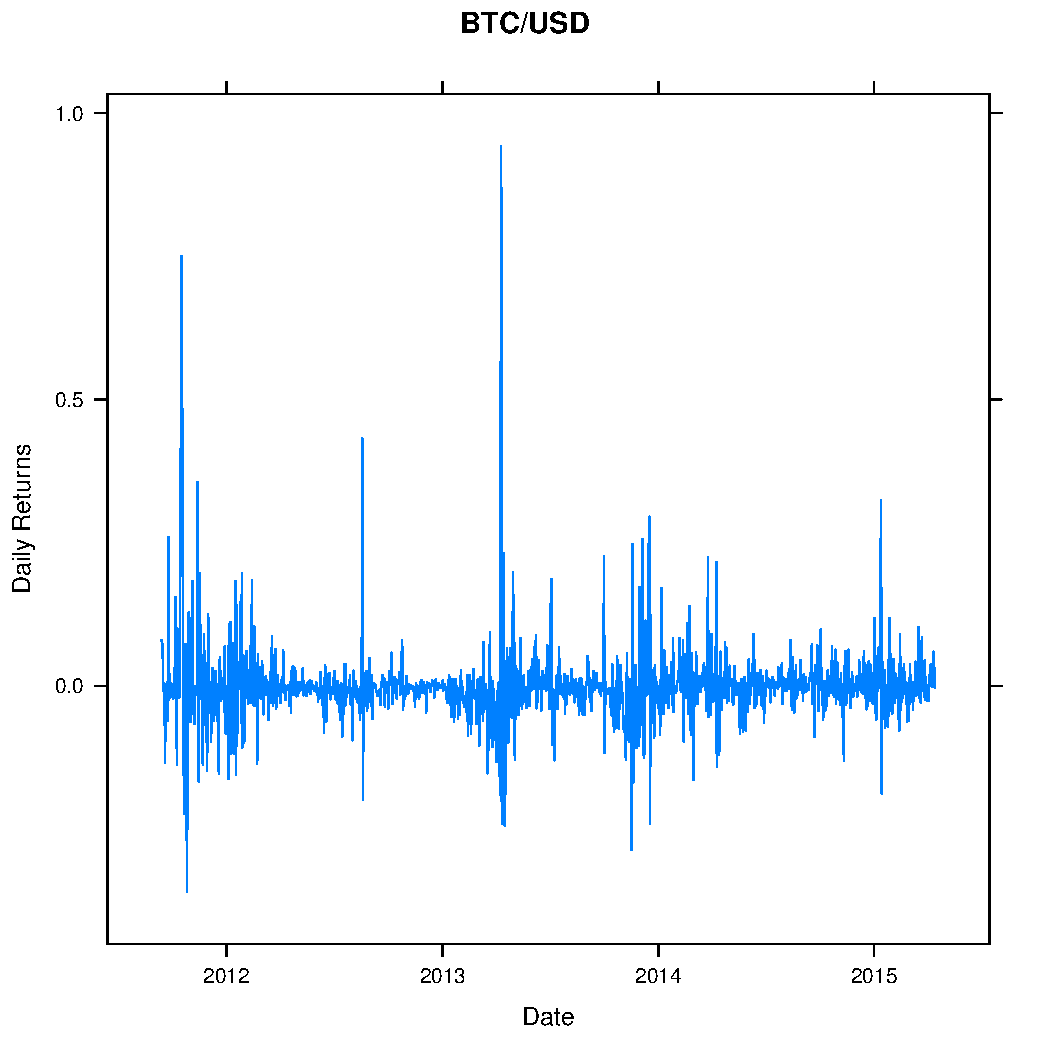
\includegraphics[keepaspectratio,width=0.75\textwidth]{btcror.pdf} 
  \end{center}
\end{frame}

\begin{frame}{Do you see a trend?}
  \begin{center}
    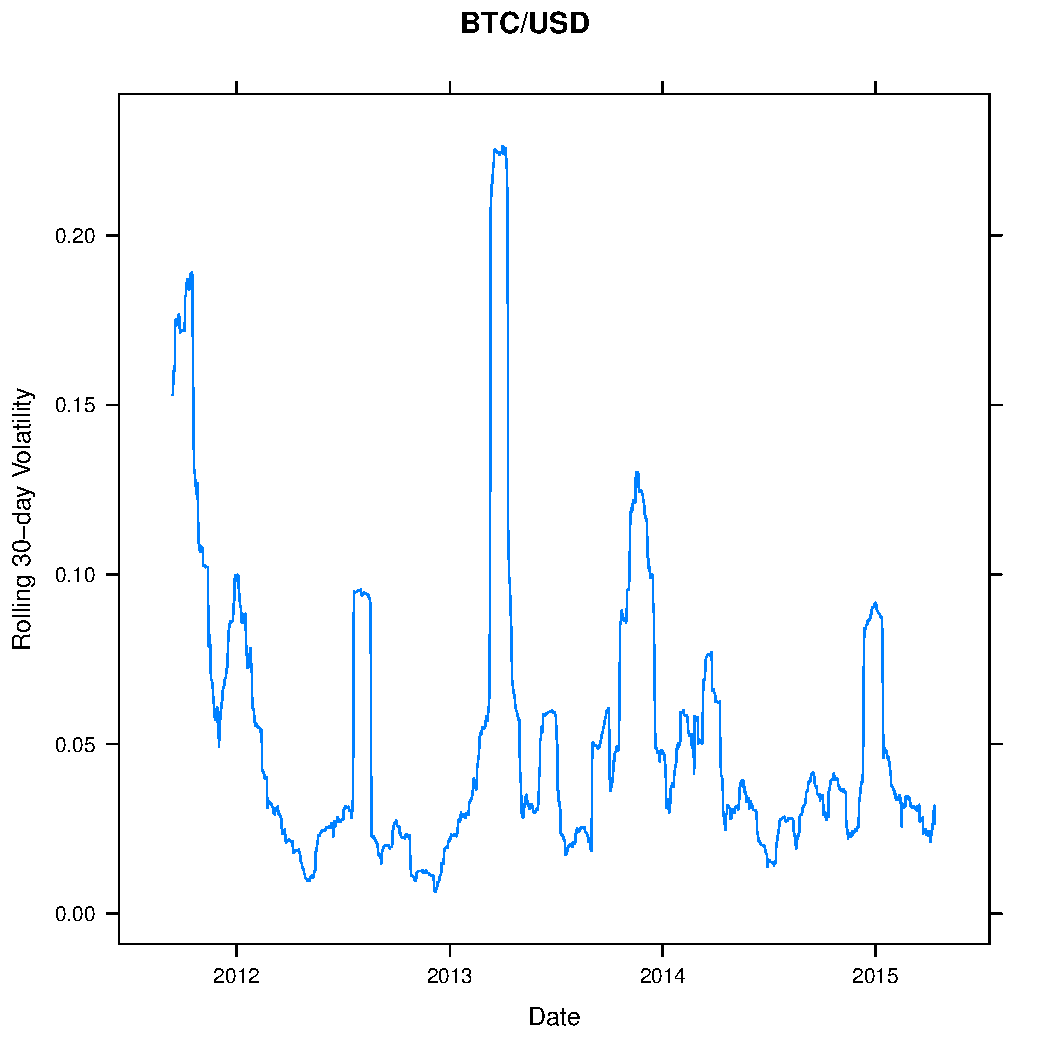
\includegraphics[keepaspectratio,width=0.75\textwidth]{btcvol.pdf} 
  \end{center}
\end{frame}

\begin{frame}
  \frametitle{Will Bitcoin Volatility Decline?}

  \begin{description}
  \item[Short answer] No.
  \item[Longer answer] No, unless future demand becomes more
    predictable.
  \end{description}
  
  And, no, a more liquid BTC market will not make Bitcoin's
  price more stable\dots

  \begin{block}{}
    \emph{The main volatility in bitcoin comes from variability in
    speculation, which in turn is due to the genuine uncertainty about
    its future. More efficient liquidity mechanisms don't help
    reduce genuine uncertainty.}\\\textbf{Nick Szabo}
  \end{block}
  
\end{frame}

\begin{frame}
  \frametitle{Deterministic Coin Supply}

  \begin{block}{What is ``deterministic coin supply''?}
    The growth rate of coin supply is completely specified in advance
    and is not influenced by facts outside of the system.
  \end{block}

  \begin{itemize}
  \item This is \emph{not} "digital gold"
  \item Even gold has a supply that responds to its price
  \item Bitcoin is more like a "digital collectable"
  \end{itemize}

\end{frame}

\begin{frame}
  \frametitle{Coin Demand}
  \begin{description}
  \item[Transactional Coin Demand $CD_{T}$] Desire to hold a certain
    quantity of coins for the purpose of making transactions.
  \item[Speculative Coin Demand $CD_{S}$] Desire to hold a certain
    quantitiy of coins to speculate on future increases in coin
    price / purchasing power. 
  \end{description}

  \begin{block}{Coin demand made up of both transactional and
      speculative motives}
    \begin{equation*}
      CD = CD_{T} + CD_{S}  
    \end{equation*}
  \end{block}
\end{frame}

\begin{frame}
  \frametitle{Coin Demand}
  \begin{block}{Coin demand is a quantity of \textbf{purchasing power}}
    \begin{equation*}
      CD = P \times Q
    \end{equation*}
    \begin{description}
    \item[$P$] purchasing power, coin price of a broad basket of goods
      and services
    \item[$Q$] quantity of coins demanded given $P$
    \end{description}
  \end{block}
\end{frame}

\begin{frame}
  \frametitle{Coin Demand Curve (and fixed supply)}
  \begin{columns}
    \column{0.6\linewidth}
    \begin{block}{$CD$ Change with Fixed Supply}
      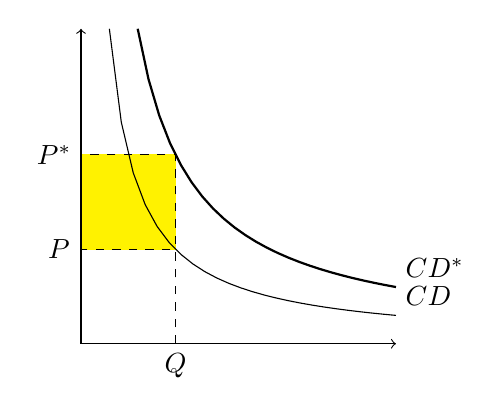
\begin{tikzpicture}[scale=0.40]
        \draw[fill=yellow,yellow] (3,3) rectangle (0,6); % yellow box
        \draw[<->] (0,10) -- (0,0) -- (10,0); % axis
        \draw[domain=0.9:10] plot (\x, {9/\x}); % CD curve
        \node[above right] at (10,0.9) {$CD$};
        \draw[thick,domain=1.8:10] plot (\x, {18/\x}); % CD* curve
        \node[above right] at (10,1.8) {$CD^{*}$};
        \draw[dashed] (3,0) -- (3,3) -- (0,3) node[left]{$P^{}$}; % marks
        \draw[dashed] (3,0) node[below]{$Q$} -- (3,6) -- 
        (0,6) node[left]{$P^{*}$};
      \end{tikzpicture}
    \end{block}
    \column{0.4\linewidth} 
    With a deterministic supply protocol like Bitcoin's, an X\%
    increase in \textbf{demand} ($CD$ to $CD^{*}$) causes an X\%
    increase in \textbf{coin price} ($P$ to $P^{*}$) because supply is
    fixed in the period.
  \end{columns}
\end{frame}

\begin{frame}
  \frametitle{Coin Demand Curve (fully elastic supply)}
  \begin{columns}
    \column{0.6\linewidth}
      \begin{block}{$CD$ Change with Elastic Supply}
        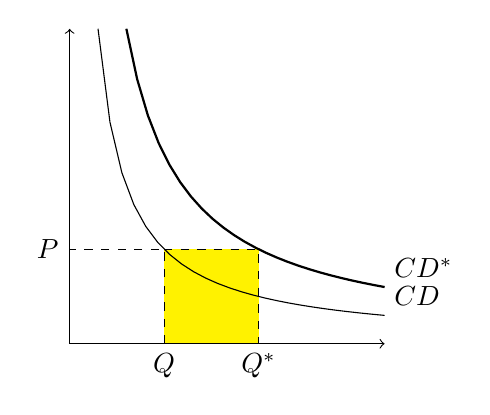
\begin{tikzpicture}[scale=0.40]
          \draw[fill=yellow,yellow] (3,3) rectangle (6,0); % yellow box
          \draw[<->] (0,10) -- (0,0) -- (10,0); % axis
          \draw[domain=0.9:10] plot (\x, {9/\x}); % CD curve
          \node[above right] at (10,0.9) {$CD$};
          \draw[thick,domain=1.8:10] plot (\x, {18/\x}); % CD* curve
          \node[above right] at (10,1.8) {$CD^{*}$};
          \draw[dashed] (3,0) node[below]{$Q$} -- (3,3) -- 
          (0,3) node[left]{$P^{}$}; % marks
          \draw[dashed] (3,3) -- (6,3) -- 
          (6,0) node[below]{$Q^{*}$};
        \end{tikzpicture}
      \end{block}
    \column{0.4\linewidth} 
    An X\% increase in \textbf{demand} ($CD$ to $CD^{*}$) causes an
    X\% increase in \textbf{coin quantity} ($Q$ to $Q^{*}$) because
    supply can change in the period.
  \end{columns}
\end{frame}

\begin{frame}
  \frametitle{Deterministic Supply Causes Volatility}
  \begin{itemize}
  \item If demand growth exceeds pre-programmed supply
    growth, coin price will increase.
  \item But if we \textbf{expect today} that this will happen in
    future, then price increase will happen today (\textbf{``Law of
      Iterated Expectations''}).
  \item Therefore, bitcoin price reflects today's expectations of
    future demand growth.
  \item \dots and deterministic supply \textbf{creates speculative
      demand} $CD_{S}$.
  \end{itemize}

  \begin{block}{A prediction market on itself}
    So bitcoin price is a like a prediction market on the growth rate
    of its own future adoption. Price volatility reflects irreducible
    uncertainty about its future. 
  \end{block}
\end{frame}

\begin{frame}
  \frametitle{``So it's like a growth stock, right?''}

  \begin{block}{}
    Transactional coin demand $CD_{T}$ is inversely related to coin
    volatility.
  \end{block}

  The more volatile the coin, the less useful it is as a medium of
  exchange.

  \begin{itemize}
  \item Volatility raises \textbf{transaction costs} for merchants.
  \item Volatility renders coin useless as a \textbf{unit-of-account}.
  \item Volatility increases need for \textbf{re-balancing}.
  \end{itemize}

  \begin{block}{No, it's not like a growth stock}
    The stock price of a young, high growth company is also
    volatile. But the volatility of the a growth company's stock
    \textbf{does \emph{not} influence the demand for its product}. But
    the volatility of bitcoin \emph{does} influence the demand for
    bitcoin as a medium-of-exchange.
  \end{block}
\end{frame}

\section{Design Goal and Two Hard Problems}

\begin{frame}
  \frametitle{Elastic Coin Supply}
  \begin{block}{Core Operational Principle}
    At the end of some pre-defined interval of time (the \emph{rebase
      period}, every $n$ blocks), if the change in coin price of the
    interval is X\%, change coin supply by X\%.
    \begin{eqnarray*}
      Q_{i} &=& Q_{i-1} \times \frac{P_{i}}{P_{i-1}}\\
      \Delta_{i} &=& Q_{i} - Q_{i-1}
    \end{eqnarray*}
    , where $i$ is the i-th rebase period, $Q$ is coin supply and $P$
    is coin price.
  \end{block}
\end{frame}

\begin{frame}
  \frametitle{Theoretical Lineage}

  \begin{block}{Bitcoin}
    \begin{itemize}
    \item Gold standard
    \item Austrian Economics  
    \end{itemize}
  \end{block}

  \begin{block}{Stablecoin}
    \begin{itemize}
    \item Milton Friedman's ``k-percent rule''
    \item Irving Fisher's ``Dollar Stabilisation''
    \end{itemize}
  \end{block}

  \begin{itemize}
  \item Both favour ``rules over discretion'' w.r.t. money
    supply.
  \item These theories assume fractional reserve banking.
  \item Differing opinions about nature of money demand.
  \item Ironically, Bitcoin gives rise to very ``Keynsian-like'' money
    demand.
  \end{itemize}
  
\end{frame}

\begin{frame}
  \frametitle{Two Hard Problems}
  \begin{enumerate}
  \item \textbf{Coin distribution}. How is $\Delta_{i}$ distributed?
  \item \textbf{Data representation}. How can $P_{i}$ be represented
    inside the network in a way that requires minimal trust?
  \end{enumerate}
\end{frame}

\begin{frame}
  \frametitle{Solution Attempt: Hayek Money}
  
  \begin{block}{Pro-rata Rule}
    Distribute $\Delta_{i}$ pro-rata over wallet balances: multiply
    each wallet balance by $Q_{i}/Q_{i-1}$.
  \end{block}
  
  \begin{block}{Why it doesn't work}
    Hayek Money only stabilises \textbf{coin price}, it doesn't stabilise
    coin \textbf{purchasing power}
  \end{block}

  Ferdinando Amertrano, \emph{Hayek Money: The Cryptocurrency Price
    Stability Solution} 
  \url{http://ssrn.com/abstract=2425270}
\end{frame}

\begin{frame}
  \frametitle{Solution Attempt: Hayek Money}

  \begin{block}{The Three Functions of Money}
    \begin{enumerate}
    \item Unit-of-Account (UoA)
    \item Store-of-Value (SoV)
    \item Medium-of-Exchange (MoE)
    \end{enumerate}
  \end{block}
  
  \begin{itemize}
  \item Price stability must stabilise both UoA and SoV. Hayek Money only
    stabilises UoA. 
  \item trades a \textbf{fixed wallet balance with fluctuating coin
      price} for a \textbf{fixed coin price with fluctuating wallet
      balance}.
  \item purchasing power of a Hayek Money wallet is just as volatile as
    a Bitcoin wallet balance.
  \item Self-defeating dynamic of $CD_{S}$ driving out $CD_{T}$ remains.
  \end{itemize}

\end{frame}

\begin{frame}
  \frametitle{Solution Attempt: Inv/Sav Wallets}

  \begin{block}{Distribute over Inv Wallets}
    Allow users to divide coin balance between ``Investment'' (Inv) and
    ``Savings'' (Sav) wallets. Distribute $\Delta_{i}$ over Inv wallets.
  \end{block}

  \begin{itemize}
  \item Solution appreciates that there must be two different vehicles
    for two different sources of coin demand: Sav Wallets for $CD_{T}$
    and Inv wallets for $CD_{S}$.
  \item $\Delta_{i}$ should apply to the $CD_{S}$ vehicle (Inv wallets)
  \end{itemize}
  
  Massimo Morini, \emph{Inv/Sav Wallets and the Role of Financial
    Intermediaries in a Digital Currency}
  \url{http://ssrn.com/abstract=2458890}

\end{frame}
  
\begin{frame}
    \frametitle{Solution Attempt: Inv/Sav Wallets}

  \begin{block}{Why it doesn't work}
    1:1 convertibility between Inv and Sav wallets means that no
    incentive at time $t$ to keep coin in Inv wallet when expectation
    is that $\Delta_{t+1} < 0$.
  \end{block}

\end{frame}

\section{Solution to Problem 1: Seigniorage Shares}

\begin{frame}
  \frametitle{We need \emph{two} coins}

  \begin{itemize}
  \item coins and shares
  \item \textbf{coins} are the object of stabilisation
  \item $\Delta_{i}$ is distributed over \textbf{shares}
  \item coins and shares exchange at a \textbf{\emph{market}} rate
  \item \textbf{shares} can be valued
  \end{itemize}

\end{frame}

\begin{frame}
  \frametitle{Creation of One Requires Distruction of the Other}
  \begin{block}{$\Delta_{i} > 1$: coin supply needs to \emph{increase}}
    \begin{itemize}
    \item Auction at end of rebase period \textbf{buying} $\Delta_{i}$
      \emph{worth of shares}; users can \textbf{offer shares}.
    \item $\Delta_{i}$ worth of shares are bought at winning
      coins-for-shares price $P^{S}$.
    \item $\Delta_{i}$ coins are \textbf{created}.
    \item $\Delta_{i}$ worth of shares are \textbf{destroyed}.
    \end{itemize}
  \end{block}

\end{frame}

\begin{frame}
  \frametitle{Creation of One Requires Distruction of the Other}
  \begin{block}{$\Delta_{i} < 1$: coin supply needs to \emph{decrease}}
      
    \begin{itemize}
    \item Auction at end of rebase period \textbf{selling} $\Delta_{i}$
      \emph{worth of shares}, users can \textbf{bid for shares}.
    \item $\Delta_{i}$ worth of shares are sold at winning
      coins-for-shares price $P^{S}$.
    \item $\Delta_{i}$ coins are \textbf{destroyed}.
    \item $\Delta_{i}$ worth of shares are \textbf{created}.
    \end{itemize}

  \end{block}

\end{frame}

\begin{frame}
  \frametitle{How do we value shares?}

  \begin{block}{Problem}
    So if long-term growth rate of $\Delta_{i}$ is positive (demand
    for coin on average grows), then shares become increasingly
    scarce. How can we value those shares? 
  \end{block}

  \begin{block}{Solution}
    Consider the following shares investment strategy where you own
    $\omega$ shares. 
    \newcommand*{\Fraction}{\lvert\frac{\Delta_{i}}{P^{s}_{i}Q^{s}_{i}}\rvert}%
    \begin{itemize}
    \item When $\Delta_{i} > 1$, \textbf{buy}
      $\Fraction \times \omega$ shares in the auction.
    \item When $\Delta_{i} < 1$, \textbf{sell}
      $\Fraction \times \omega$ shares in the auction.
    \end{itemize}
  \end{block}

\end{frame}

\begin{frame}
  \frametitle{What has this strategy done?}

  Share owner maintains a position that is a \textbf{constant
    percentage} of the outstanding share supply. Therefore, his
  investment is a claim on a constant percentage of $\Delta_{i},
  \Delta_{i+1}, \Delta_{i+2}, \dots$ coin-denominated \textbf{cash
    flows}.

  \begin{center}
    \textbf{Valuation is a simple Net Present Value (NPV)!!!}
  \end{center}

  \begin{block}{Fair Value of Shares}
    \begin{equation*}
      P^{s}_{t} = \frac{1}{Q^{s}_{t}}\sum\limits_{i=t}^{\infty}\frac{\Delta_{i}}{(1+r_{i})^{i}}
    \end{equation*}
  \end{block}
  Shares are like equity, where the income is coin seigniorage. Hence
  the name \emph{\textbf{Seigniorage Shares}}.
\end{frame}

\begin{frame}
  \frametitle{The Monetary Yin-Yang}

  \begin{columns}

    \column{0.7\linewidth}
    \begin{description}
    \item[Coins] Call them \textbf{\emph{Yin}}. Caters to $CD_{T}$,
      \dots stable, feminine, risk-averse.
    \item[Shares] Call them \textbf{\emph{Yang}}. Caters to $CD_{S}$,
      \dots volatile, masculine, risk-taking.
    \end{description}

    \column{0.3\linewidth}
    \begin{center}
      
\includegraphics[scale=0.3]{yinyang.png}  
    \end{center}
  \end{columns}

  \begin{itemize}
  \item Stable coins need shares to absorbe periods of declining coin
    demand, to assume the risk of unpredictable changes in money
    demand.
  \item Shares need stable coins to generate demand growth in the
    first place.
  \item So $CD_{T}$ and $CD_{S}$ reinforce each other under the
    monetary yin-yang of seigniorage shares, but undermine each other
    under the "barbarous relic" of fixed coin supply (eg Bitcoin).
  \end{itemize}

\end{frame}

\begin{frame}
  \frametitle{Problems and Questions}
  
  \begin{itemize}
  \item What happens when $CD$ growth rate slows and ratio of shares
    market value to coin market value goes from $>1$ to $<1$?
  \item Is it possible for coin to devalue in an orderly way?
  \item Any market manipulation vectors implicit in auction design?
  \end{itemize}

\end{frame}

\section{Solutions to Problem 2}

\begin{frame}
  \frametitle{Strategies for Modelling Coin Value}

  \begin{block}{Exogenous Solutions}

    \begin{itemize}
    \item Trusted oracles
      \begin{itemize}
      \item "but I thought cryptocurrency was supposed to be
        autonomous of any trusted third-parties"
      \end{itemize}
    \item Schelling games
      \begin{itemize}
      \item is truth really a Schelling point?
      \end{itemize}
    \end{itemize}

  \end{block}

  \begin{block}{Endogenous Solutions}

    \begin{itemize}
    \item Transaction volume 
      \begin{itemize}
      \item assumes stable money velocity
      \item subject to manipulation
      \end{itemize}
    \item \textbf{Difficulty-based estimators}
      \begin{itemize}
      \item Promising strategy! See estimator research by Vitalik
        Buterin
        \url{https://github.com/ethereum/economic-modeling/tree/master/stability}
      \end{itemize}
    \end{itemize}

  \end{block}
  
\end{frame}

\begin{frame}
  \frametitle{Restricting Schelling Game to Shareholders}

  \begin{itemize}
  \item What if only shareholders could play the Shelling game,
    perhaps pro-rata their percentage of share ownership? Does
  \item We can prove that shareholders do not have an incentive
    w.r.t. their shareholdings to submit dishonest coin
    valuations. Exaggerating the supply of coin that needs to increase
    does increase NPV of share price in coin-denominated terms, but no
    effect on real share price.
  \item Arguably, expectations of real coin demand will decline with
    dishonest coin valuations, so shareholders have an incentive
    w.r.t. share wealth to vote the truth. 
  \end{itemize}

\end{frame}

\begin{frame}
  \frametitle{Restricting Schelling Game to Shareholders}

  \begin{alertblock}{This was done late at night}
    \dots so the following may contain errors!! 
  \end{alertblock}

  Simplify the set-up a bit (hopefully, without loss of generality)
  and say that the expected demand growth for coin is $g$, so 
  \begin{equation}
    \Delta_{t} = \Delta_{t-1}(1+g)
  \end{equation}
  , where $g<r$ and the valuation model from previous slide can be
  defined in terms of $g$ and $r$:
  \begin{eqnarray}
    P^{s}_{t} &=&
    \frac{1}{Q^{s}_{t}}\sum\limits_{i=t}^{\infty}\frac{\Delta_{i}}{(1+r_{i})^{i}}\\
            &=& \frac{1}{Q^{s}_{t}}\frac{\Delta_{t}}{r-g}
  \end{eqnarray}

\end{frame}

    
\begin{frame}
  \frametitle{Restricting Schelling Game to Shareholders}

  \begin{block}{Question}
    If shareholders had the power to represent coin price $P_{i}$ to
    the network, do they have an incentive to be untruthful
    w.r.t. their share wealth?
  \end{block}
  
  \begin{itemize}
  \item Let $\rho_{i}$ be the true market value of the coin index and let
    $\epsilon = P_{i}/\rho_{i}$ be the measure of untruthfullness.
  \item It might be argued shareholders have incentive to make
    $\epsilon$ large, exagerate value of coin in order to squeeze more
    seigniorage out of system.
  \end{itemize}

\end{frame}

\begin{frame}
  \frametitle{Restricting Schelling Game to Shareholders}

  \begin{block}{Implication for coin price}
    If we hold $CD$ constant, then a non-zero $\epsilon$ will cause
    the actual coin value $\hat{P}_{t}$ to change to:
    \begin{equation}
      \hat{P}_{t} = P_{t}\frac{1}{\epsilon}
    \end{equation}
  \end{block}

  \begin{block}{Implication for share price}
    \begin{equation}
      \hat{P}^{s}_{t} = P^{s}_{t}\epsilon
    \end{equation}
  \end{block}
\end{frame}

\section{Alternative Approach: SchellingDollar}

\begin{frame}
  \frametitle{Vitalik Buterin's SchellingDollar Model}
  \begin{itemize}
  \item Two currencies, \emph{vol-coins} (V) and \emph{stable-coins} (S)
  \item Can only hold 0 or positive balance of V
  \item Can hold negative or postive balance of S. But negative
    balance of S requires quantity of V equal in value to 2X their new
    S balance. 
    \begin{example}
      If S is \$1 and V is \$5, then if user has 10V (\$50) they can
      at most reduce their S balance to -25.
    \end{example}
  \item If value of user's negative S exceeds 90\% of the value of
    user's V, then user's S and V balances are both reduced to
    zero. (implication for total V supply)
  \end{itemize}
\end{frame}


\begin{frame}
  \frametitle{Vitalik Buterin's SchellingDollar Model}

  \begin{itemize}
  \item Can convert between S and V at a rate of \$1 worth of V per
    S, plus a small exchange fee (implication for total V supply)
  \item System keeps track of total +S and -S in circulation.
  \item If $\frac{+S}{-S} > 1$, system imposes a negative interest rate on all
    V to make +S holdings less attractive and -S holdings more
    attractive.
  \item If $\frac{+S}{-S} < 1$, system imposes a positive interest rate on all
    V to make -S holdings less attractive and +S holdings more
    attractive.
  \end{itemize}
\end{frame}

\begin{frame}
  \frametitle{How Do We Value V in SchellingDollar Model?}

  \begin{itemize}
  \item As with Seigniorage shares, all changes in +S demand are V's
    ``income''.
  \item V profits from TX fees for exchanging V and S.
  \end{itemize}

  \begin{block}{Additional Profit/Loss for V}
    \begin{itemize}
    \item increase in V price and $\frac{+S}{-S} > 1 \rightarrow$ decrease V supply
    \item decrease in V price and $\frac{+S}{-S} > 1 \rightarrow$ increase V supply
    \item increase in V price and $\frac{+S}{-S} < 1 \rightarrow$ increase V supply
    \item decrease in V price and $\frac{+S}{-S} < 1 \rightarrow$ decrease V supply
    \end{itemize}
  \end{block}

\end{frame}

\begin{frame}
  \frametitle{Some Problems/Questions with SchellingDollar}
  
  \begin{itemize}
  \item Pro-cyclical interest rate\dots what implications does this
    have for expectations of long-term +S demand growth?
  \item Negative correlation between V price changes and
    $\frac{+S}{-S}$.
  \end{itemize}

  \begin{block}{Correlation Drag?}
    If correlation between V price changes and $\frac{+S}{-S}$ is
    negative, then this acts as a tax on V\dots lowers its fair
    value. Reasons why correlation might be negative:
    \begin{itemize}
    \item Rebalancing\dots -S holders must buy V when price goes up
      and sell V when price goes down to keep leverage ratio
      constant.
    \item Serial correlation in V price. Reasonable to predict demand
      for leveraged V positions higher in a bull market than in a bear
      market. 
    \end{itemize}
  \end{block}

\end{frame}

\end{document}


